\documentclass[12pt,letterpaper]{article}\usepackage[]{graphicx}\usepackage[]{color}
%% maxwidth is the original width if it is less than linewidth
%% otherwise use linewidth (to make sure the graphics do not exceed the margin)
\makeatletter
\def\maxwidth{ %
  \ifdim\Gin@nat@width>\linewidth
    \linewidth
  \else
    \Gin@nat@width
  \fi
}
\makeatother

\definecolor{fgcolor}{rgb}{0.345, 0.345, 0.345}
\newcommand{\hlnum}[1]{\textcolor[rgb]{0.686,0.059,0.569}{#1}}%
\newcommand{\hlstr}[1]{\textcolor[rgb]{0.192,0.494,0.8}{#1}}%
\newcommand{\hlcom}[1]{\textcolor[rgb]{0.678,0.584,0.686}{\textit{#1}}}%
\newcommand{\hlopt}[1]{\textcolor[rgb]{0,0,0}{#1}}%
\newcommand{\hlstd}[1]{\textcolor[rgb]{0.345,0.345,0.345}{#1}}%
\newcommand{\hlkwa}[1]{\textcolor[rgb]{0.161,0.373,0.58}{\textbf{#1}}}%
\newcommand{\hlkwb}[1]{\textcolor[rgb]{0.69,0.353,0.396}{#1}}%
\newcommand{\hlkwc}[1]{\textcolor[rgb]{0.333,0.667,0.333}{#1}}%
\newcommand{\hlkwd}[1]{\textcolor[rgb]{0.737,0.353,0.396}{\textbf{#1}}}%

\usepackage{framed}
\makeatletter
\newenvironment{kframe}{%
 \def\at@end@of@kframe{}%
 \ifinner\ifhmode%
  \def\at@end@of@kframe{\end{minipage}}%
  \begin{minipage}{\columnwidth}%
 \fi\fi%
 \def\FrameCommand##1{\hskip\@totalleftmargin \hskip-\fboxsep
 \colorbox{shadecolor}{##1}\hskip-\fboxsep
     % There is no \\@totalrightmargin, so:
     \hskip-\linewidth \hskip-\@totalleftmargin \hskip\columnwidth}%
 \MakeFramed {\advance\hsize-\width
   \@totalleftmargin\z@ \linewidth\hsize
   \@setminipage}}%
 {\par\unskip\endMakeFramed%
 \at@end@of@kframe}
\makeatother

\definecolor{shadecolor}{rgb}{.97, .97, .97}
\definecolor{messagecolor}{rgb}{0, 0, 0}
\definecolor{warningcolor}{rgb}{1, 0, 1}
\definecolor{errorcolor}{rgb}{1, 0, 0}
\newenvironment{knitrout}{}{} % an empty environment to be redefined in TeX

\usepackage{alltt}
\usepackage[utf8]{inputenc}
\usepackage[margin=.7in]{geometry}
\usepackage{graphicx}
\usepackage{titling}
\usepackage{amsmath}
\usepackage{amsfonts}
\usepackage{amssymb}
\renewcommand{\theenumiv}{\arabic{enumiv}}
\setlength{\droptitle}{-5em}
\author{Maurice Diesendruck}
\title{StatMod2 - Exercises 5 - PCA - Question 3 - Congress Data}
\IfFileExists{upquote.sty}{\usepackage{upquote}}{}
\begin{document}
\maketitle
\setcounter{section}{3}

\subsection{Evaluation of First Principal Component}

  Using "congress109.csv" and "congress109members.csv", project data onto first
  principal component (i.e. get vector $Z=Yv_1$, where $v_1$ is the first column 
  of the right-singular matrix of $Y=U \Sigma V'$). Then, merge with data about
  people, and identify relationships. A \texttt{pairs.panels} output is 
  displayed.
  
  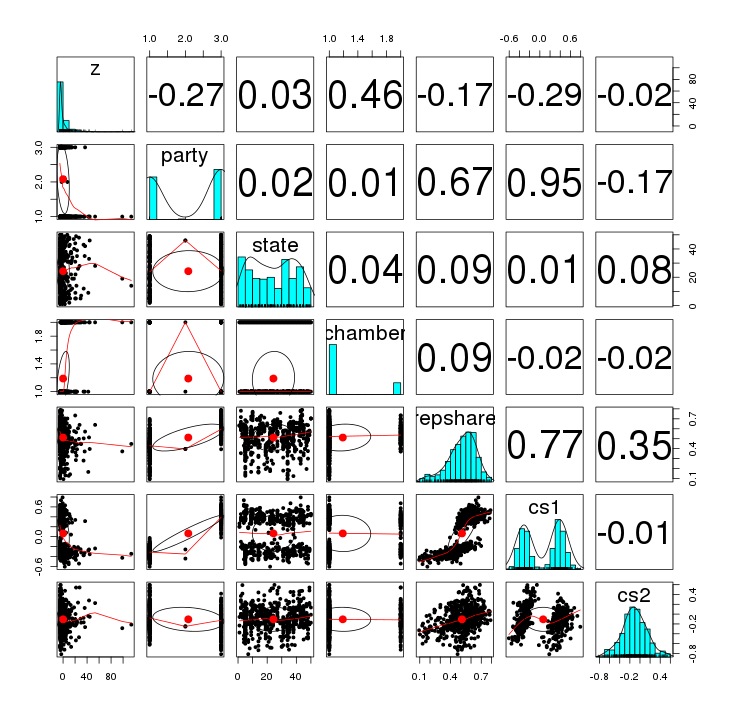
\includegraphics[width=.9\textwidth, keepaspectratio]{pca-pairs-panels.png}
  
  The first principal component appears to be most strongly related to 
  \texttt{chamber}, where a higher $z$ is associated with being in the smaller
  chamber (presumed to be the "senate", versus the "house").
  
\newpage
\subsection{Rank $k$ Approximation. Which $k$?}

  Each principal component accounts for a portion of the overall variance. What
  should $k$ be for a rank-$k$ approximation? One heuristic is to choose $k$ so
  that the cumulative sum of those $k$ variances is 80\% of the total variance.
  The following graph shows that for this data set, $k=50$.\\
  \begin{center}
  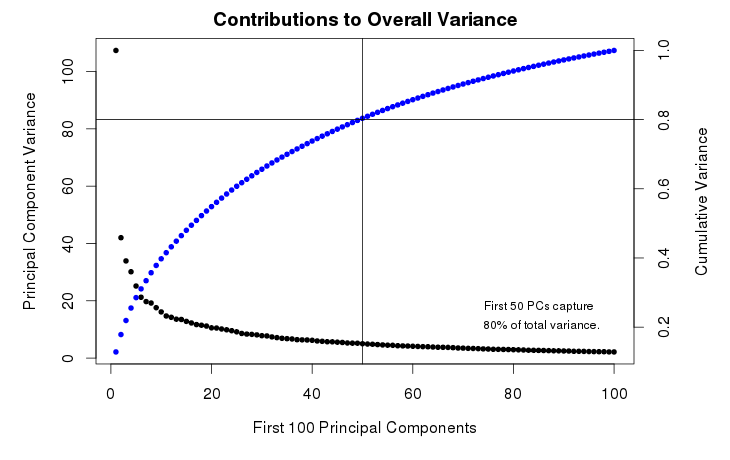
\includegraphics[width=.7\textwidth, keepaspectratio]
    {pca-cumulative-variance.png}
  \end{center}

\subsection{Comparing Lower-Rank Approximations Using Frobenius Norm}

  The Frobenius norm can measure how close the rank-$k$ approximation is to the 
  original data matrix. Results are shown below, demonstrating that including
  more principal components generally improves "closeness" to the original data.
  
  \begin{center}
  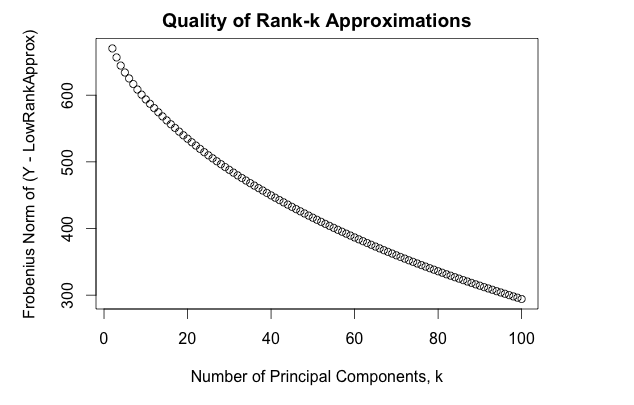
\includegraphics[width=.7\textwidth, keepaspectratio]{pca-frobenius.png}
  \end{center}

\newpage
\subsection{Full R Code}

\begin{knitrout}
\definecolor{shadecolor}{rgb}{0.969, 0.969, 0.969}\color{fgcolor}\begin{kframe}
\begin{alltt}
\hlcom{# StatMod2 - Latent Feature Models (PCA)}

\hlkwd{library}\hlstd{(Matrix)}
\hlkwd{library}\hlstd{(psych)}

\hlstd{data} \hlkwb{<-} \hlkwd{read.csv}\hlstd{(}\hlstr{"congress109.csv"}\hlstd{)}
\hlstd{data2} \hlkwb{<-} \hlkwd{read.csv}\hlstd{(}\hlstr{"congress109members.csv"}\hlstd{)}

\hlcom{# Remove column of names.}
\hlstd{Y} \hlkwb{<-} \hlkwd{as.matrix}\hlstd{(data[,}\hlopt{-}\hlnum{1}\hlstd{])}
\hlstd{n} \hlkwb{<-} \hlkwd{dim}\hlstd{(Y)[}\hlnum{1}\hlstd{]}
\hlstd{p} \hlkwb{<-} \hlkwd{dim}\hlstd{(Y)[}\hlnum{2}\hlstd{]}
\hlkwd{names}\hlstd{(Y)} \hlkwb{<-} \hlkwd{seq}\hlstd{(}\hlnum{1}\hlopt{:}\hlkwd{dim}\hlstd{(Y)[}\hlnum{2}\hlstd{])} \hlcom{# Enables compact printing.}
\hlcom{# Standardize columns of Y to be mean=0, sd=1.}
\hlkwa{for} \hlstd{(c} \hlkwa{in} \hlnum{1}\hlopt{:}\hlstd{p) \{}
  \hlstd{Y[,c]} \hlkwb{<-} \hlstd{(Y[,c]} \hlopt{-} \hlkwd{mean}\hlstd{(Y[,c]))}\hlopt{/}\hlkwd{sqrt}\hlstd{(}\hlkwd{var}\hlstd{(Y[,c]))}
\hlstd{\}}

\hlcom{# Do SVD of Y.}
\hlstd{decomp.y} \hlkwb{<-} \hlkwd{svd}\hlstd{(Y)}
\hlstd{U.y} \hlkwb{<-} \hlkwd{as.matrix}\hlstd{(decomp.y}\hlopt{$}\hlstd{u)}
\hlstd{D.y} \hlkwb{<-} \hlkwd{as.matrix}\hlstd{(}\hlkwd{diag}\hlstd{(decomp.y}\hlopt{$}\hlstd{d))}
\hlstd{V.y} \hlkwb{<-} \hlkwd{as.matrix}\hlstd{(decomp.y}\hlopt{$}\hlstd{v)}

\hlcom{# Do eigenvalue decomposition of S=(1/n)*t(Y)*Y}
\hlstd{S1} \hlkwb{<-} \hlkwd{cov}\hlstd{(Y)}
\hlstd{S} \hlkwb{<-} \hlstd{(}\hlnum{1}\hlopt{/}\hlstd{n)}\hlopt{*}\hlkwd{t}\hlstd{(Y)}\hlopt\hlstd{Y}
\hlkwd{colnames}\hlstd{(S)} \hlkwb{<-} \hlkwd{seq}\hlstd{(}\hlnum{1}\hlopt{:}\hlkwd{dim}\hlstd{(S)[}\hlnum{2}\hlstd{])} \hlcom{# Enables compact printing.}
\hlkwd{rownames}\hlstd{(S)} \hlkwb{<-} \hlkwd{seq}\hlstd{(}\hlnum{1}\hlopt{:}\hlkwd{dim}\hlstd{(S)[}\hlnum{2}\hlstd{])}
\hlstd{decomp.s} \hlkwb{<-} \hlkwd{eigen}\hlstd{(S)}
\hlstd{vals.s} \hlkwb{<-} \hlstd{decomp.s}\hlopt{$}\hlstd{values}
\hlstd{vecs.s} \hlkwb{<-} \hlstd{decomp.s}\hlopt{$}\hlstd{vectors}

\hlcom{# Project all values onto 1st column of V.}
\hlstd{z} \hlkwb{<-} \hlstd{Y}\hlopt\hlstd{vecs.s[,}\hlnum{1}\hlstd{]}
\hlstd{pc1.in.context} \hlkwb{<-} \hlkwd{cbind}\hlstd{(z, data2[}\hlnum{2}\hlopt{:}\hlnum{7}\hlstd{])}
\hlkwd{pairs.panels}\hlstd{(pc1.in.context)}

\hlcom{# Test variance of projections using first 100 columns of V.}
\hlstd{range} \hlkwb{<-} \hlnum{1}\hlopt{:}\hlnum{100}
\hlstd{t} \hlkwb{<-} \hlkwa{NULL}
\hlstd{cumulative.vars} \hlkwb{<-} \hlkwa{NULL}
\hlkwa{for} \hlstd{(i} \hlkwa{in} \hlstd{range) \{}
  \hlstd{t} \hlkwb{<-} \hlkwd{c}\hlstd{(t,} \hlkwd{var}\hlstd{(Y}\hlopt\hlstd{vecs.s[,i]))}
  \hlstd{cumulative.vars[i]} \hlkwb{<-} \hlkwd{sum}\hlstd{(t[}\hlnum{1}\hlopt{:}\hlstd{i])}
\hlstd{\}}
\hlstd{cumulative.vars.scaled} \hlkwb{<-} \hlstd{cumulative.vars}\hlopt{/}\hlkwd{max}\hlstd{(cumulative.vars)}
\hlstd{pc.cutoff} \hlkwb{<-} \hlkwd{min}\hlstd{(}\hlkwd{which}\hlstd{(cumulative.vars.scaled}\hlopt{>}\hlnum{0.8}\hlstd{))}

\hlcom{# Plot cumulative variance.}
\hlkwd{par}\hlstd{(}\hlkwc{mar} \hlstd{=} \hlkwd{c}\hlstd{(}\hlnum{5}\hlstd{,}\hlnum{5}\hlstd{,}\hlnum{2}\hlstd{,}\hlnum{5}\hlstd{))}
\hlkwd{plot}\hlstd{(range, t,} \hlkwc{ylab}\hlstd{=}\hlstr{"Principal Component Variance"}\hlstd{,}
     \hlkwc{xlab}\hlstd{=}\hlkwd{bquote}\hlstd{(}\hlstr{"First"}\hlopt{~}\hlkwd{.}\hlstd{(}\hlkwd{length}\hlstd{(range))}\hlopt{~}\hlstr{"Principal Components"}\hlstd{),}
     \hlkwc{main}\hlstd{=}\hlstr{"Contributions to Overall Variance"}\hlstd{)}
\hlkwd{text}\hlstd{(}\hlnum{85}\hlstd{,} \hlnum{15}\hlstd{,} \hlkwc{cex}\hlstd{=}\hlnum{.75}\hlstd{,}
     \hlkwd{bquote}\hlstd{(}\hlkwd{atop}\hlstd{(}\hlstr{"First"}\hlopt{~}\hlkwd{.}\hlstd{(pc.cutoff)}\hlopt{~}\hlstr{"PCs capture"}\hlstd{,}
                 \hlstr{"  80% of total variance."}\hlstd{)))}
\hlkwd{par}\hlstd{(}\hlkwc{new} \hlstd{= T)}
\hlkwd{plot}\hlstd{(range, cumulative.vars.scaled,}
     \hlkwc{col} \hlstd{=} \hlstr{"blue"}\hlstd{,} \hlkwc{axes} \hlstd{= F,} \hlkwc{xlab} \hlstd{=} \hlnum{NA}\hlstd{,} \hlkwc{ylab} \hlstd{=} \hlnum{NA}\hlstd{)}
\hlkwd{axis}\hlstd{(}\hlkwc{side} \hlstd{=} \hlnum{4}\hlstd{)}
\hlkwd{mtext}\hlstd{(}\hlkwc{side} \hlstd{=} \hlnum{4}\hlstd{,} \hlkwc{line} \hlstd{=} \hlnum{3}\hlstd{,} \hlstr{"Cumulative Variance"}\hlstd{)}
\hlkwd{abline}\hlstd{(}\hlkwc{h}\hlstd{=}\hlnum{0.8}\hlstd{)}
\hlkwd{abline}\hlstd{(}\hlkwc{v}\hlstd{=pc.cutoff)}

\hlcom{# Get a lower-rank approximation of Y, using the top eigenvalues that describe}
\hlcom{# 80% of the total variance.}
\hlstd{LowRankApprox} \hlkwb{<-} \hlkwa{function}\hlstd{(}\hlkwc{U.y}\hlstd{,} \hlkwc{D.y}\hlstd{,} \hlkwc{V.y}\hlstd{,} \hlkwc{pc.cutoff}\hlstd{) \{}
  \hlstd{lr.U} \hlkwb{<-} \hlstd{U.y[,}\hlnum{1}\hlopt{:}\hlstd{pc.cutoff]}
  \hlstd{lr.D} \hlkwb{<-} \hlstd{D.y[}\hlnum{1}\hlopt{:}\hlstd{pc.cutoff,}\hlnum{1}\hlopt{:}\hlstd{pc.cutoff]}
  \hlstd{lr.V} \hlkwb{<-} \hlstd{V.y[,}\hlnum{1}\hlopt{:}\hlstd{pc.cutoff]}
  \hlstd{lr.Y} \hlkwb{<-} \hlstd{lr.U}\hlopt\hlstd{lr.D}\hlopt\hlkwd{t}\hlstd{(lr.V)}
  \hlkwd{return} \hlstd{(lr.Y)}
\hlstd{\}}

\hlcom{# Compute difference between original and low-rank approximation of Y.}
\hlstd{frob.dist} \hlkwb{<-} \hlkwa{NULL}
\hlkwa{for} \hlstd{(c} \hlkwa{in} \hlnum{2}\hlopt{:}\hlnum{100}\hlstd{) \{}
  \hlstd{lr.approx} \hlkwb{<-} \hlkwd{LowRankApprox}\hlstd{(U.y, D.y, V.y, c)}
  \hlstd{frob.dist[c]} \hlkwb{<-} \hlkwd{norm}\hlstd{(Y}\hlopt{-}\hlstd{lr.approx)}
\hlstd{\}}
\hlkwd{plot}\hlstd{(}\hlnum{2}\hlopt{:}\hlnum{100}\hlstd{, frob.dist[}\hlnum{2}\hlopt{:}\hlnum{100}\hlstd{],} \hlkwc{xlab}\hlstd{=}\hlstr{"Number of Principal Components, k"}\hlstd{,}
     \hlkwc{ylab}\hlstd{=}\hlstr{"Frobenius Norm of (Y - LowRankApprox)"}\hlstd{,}
     \hlkwc{main}\hlstd{=}\hlstr{"Quality of Rank-k Approximations"}\hlstd{)}
\end{alltt}
\end{kframe}
\end{knitrout}

\end{document}
